\documentclass[tikz,border=10pt]{standalone}
\usepackage{tikz}

\begin{document}
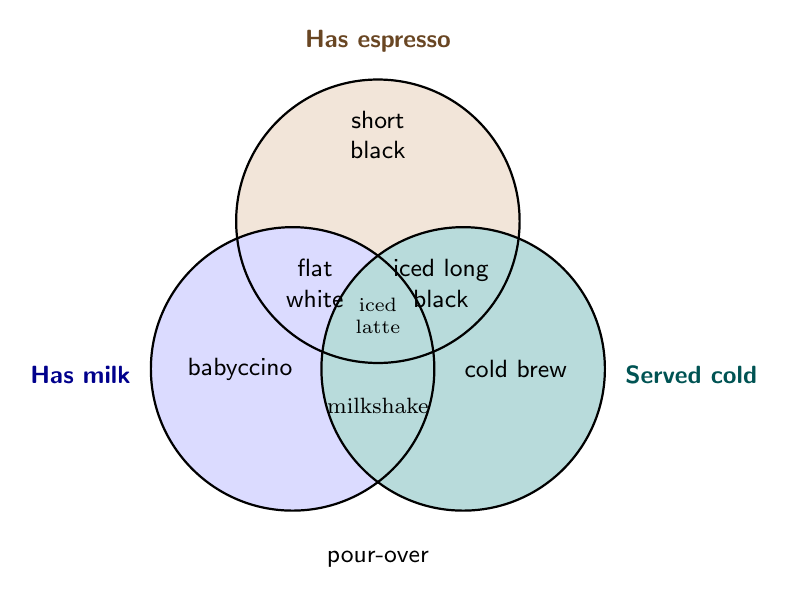
\begin{tikzpicture}[
    font=\sffamily\small,
    every node/.style={align=center, inner sep=1pt},
  ]

  % ---- circle geometry --------------------------------------------------
  % Espresso  : (0, 1.25)
  % Milk      : (-1.083, -0.625)
  % Cold      : ( 1.083, -0.625)
  % radius    : 1.8
  \def\r{1.8}

  % ---- filled discs (light tints so labels stay readable) --------------
  \fill[brown!20]  (0,1.25)         circle (\r);
  \fill[blue!14]   (-1.083,-0.625)  circle (\r);
  \fill[teal!28]   (1.083,-0.625)   circle (\r);

  \draw[thick] (0,1.25)         circle (\r);
  \draw[thick] (-1.083,-0.625)  circle (\r);
  \draw[thick] (1.083,-0.625)   circle (\r);

  % ---- set titles -------------------------------------------------------
  \node[font=\sffamily\bfseries\small, text=brown!55!black, anchor=south]
       at (0,3.35)       {Has espresso};
  \node[font=\sffamily\bfseries\small, text=blue!55!black, anchor=east]
       at (-3.1,-0.7)    {Has milk};
  \node[font=\sffamily\bfseries\small, text=teal!65!black, anchor=west]
       at (3.1,-0.7)     {Served cold};

  % ---- members ----------------------------------------------------------
  \node at (0,2.35)                      {short\\black};        % espresso only
  \node at (-0.80,0.46)                  {flat\\white};         % espresso + milk
  \node at (0.80,0.46)                   {iced long\\black};    % espresso + cold
  \node[font=\scriptsize]   at (0,0.05)   {iced\\latte};         % all three
  \node at (-1.75,-0.625)                {babyccino};           % milk only
  \node at (1.75,-0.625)                 {cold brew};           % cold only
  \node[font=\footnotesize] at (0,-1.10) {milkshake};            % milk + cold
  \node at (0,-3.05)                     {pour-over};           % none of the three

\end{tikzpicture}
\end{document}
